% Digital Logic Report Template
% Created: 2020-01-10, John Miller

%==========================================================
%=========== Document Setup  ==============================

% Formatting defined by class file
\documentclass[11pt]{article}

% ---- Document formatting ----
\usepackage[margin=1in]{geometry}	% Narrower margins
\usepackage{booktabs}				% Nice formatting of tables
\usepackage{graphicx}				% Ability to include graphics

%\setlength\parindent{0pt}	% Do not indent first line of paragraphs 
\usepackage[parfill]{parskip}		% Line space b/w paragraphs
%	parfill option prevents last line of pgrph from being fully justified

% Parskip package adds too much space around titles, fix with this
\RequirePackage{titlesec}
\titlespacing\section{0pt}{8pt plus 4pt minus 2pt}{3pt plus 2pt minus 2pt}
\titlespacing\subsection{0pt}{4pt plus 4pt minus 2pt}{-2pt plus 2pt minus 2pt}
\titlespacing\subsubsection{0pt}{2pt plus 4pt minus 2pt}{-6pt plus 2pt minus 2pt}

% ---- Hyperlinks ----
\usepackage[colorlinks=true,urlcolor=blue]{hyperref}	% For URL's. Automatically links internal references.

% ---- Code listings ----
\usepackage{listings} 					% Nice code layout and inclusion
\usepackage[usenames,dvipsnames]{xcolor}	% Colors (needs to be defined before using colors)

% Define custom colors for listings
\definecolor{listinggray}{gray}{0.98}		% Listings background color
\definecolor{rulegray}{gray}{0.7}			% Listings rule/frame color

% Style for Verilog
\lstdefinestyle{Verilog}{
	language=Verilog,					% Verilog
	backgroundcolor=\color{listinggray},	% light gray background
	rulecolor=\color{blue}, 			% blue frame lines
	frame=tb,							% lines above & below
	linewidth=\columnwidth, 			% set line width
	basicstyle=\small\ttfamily,	% basic font style that is used for the code	
	breaklines=true, 					% allow breaking across columns/pages
	tabsize=3,							% set tab size
	commentstyle=\color{gray},	% comments in italic 
	stringstyle=\upshape,				% strings are printed in normal font
	showspaces=false,					% don't underscore spaces
}

% How to use: \Verilog[listing_options]{file}
\newcommand{\Verilog}[2][]{%
	\lstinputlisting[style=Verilog,#1]{#2}
}




%======================================================
%=========== Body  ====================================
\begin{document}

\title{ELC 2137 Lab 10: 7-segment Display with Time-Division Multiplexing}
\author{Mariah Montgomery}

\maketitle


\section*{Summary}

We expanded on lab nine in this lab and made a small calculator using the switches, buttons, LEDs, and seven-segment display on a Basys board. We first created a counter that counts to four so quickly that it lights each digit on the seven segment display without flickering. Next, we created a two's complement source that converted a number to two's complement so that our final calculator could perform simple mathematical calculations. Lastly, we combined modules from our past labs and the two we created for lab 10 to complete our calculator.  


\section*{Q\&A}

\begin{enumerate}
	\item The N value that accomplished the full strength display was N=20.
\end{enumerate}


\section*{Results}

\begin{enumerate}
	
	\item Counter Test Simulation
	
	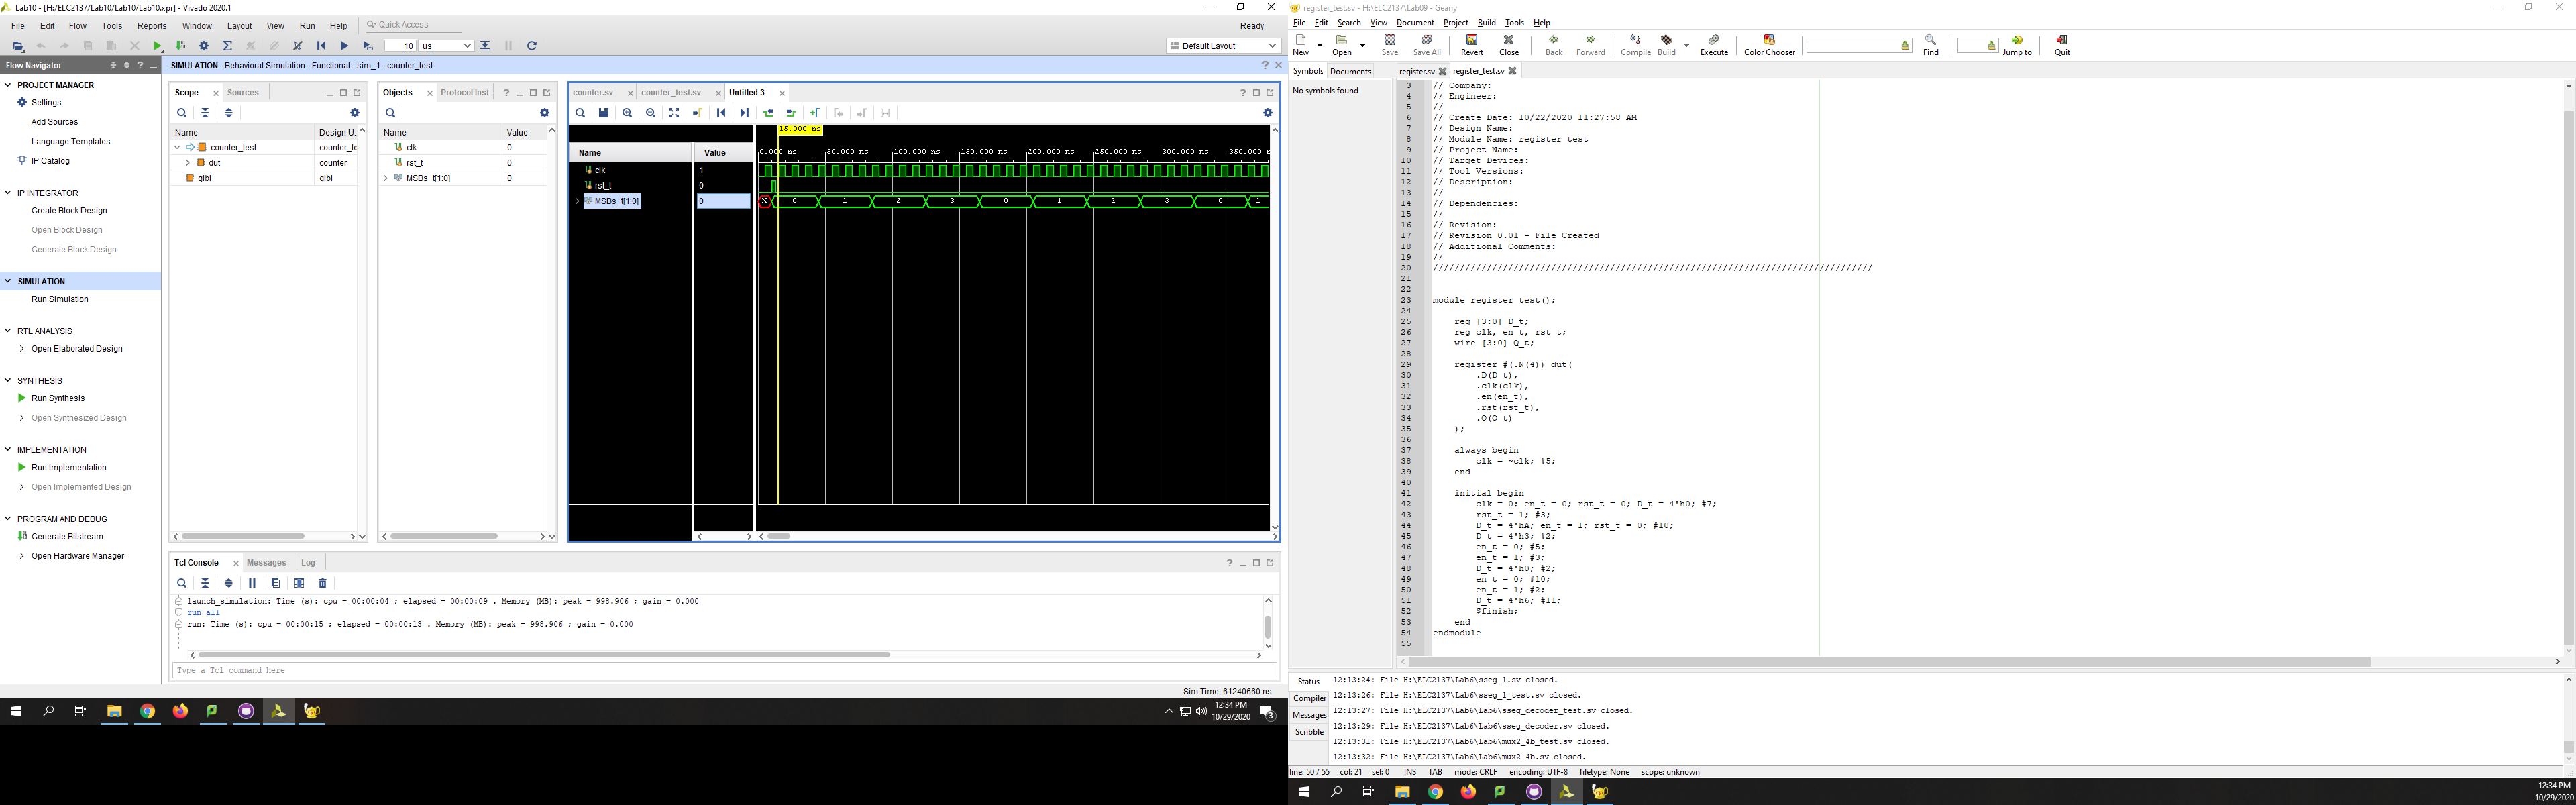
\includegraphics[width=0.8\textwidth, trim= 28.5cm 16cm 68cm 5.5cm, clip]{counter_test.PNG}
	\label{fig:Counter Test Simulation}
	
	\pagebreak
	
	\item Show 2's Complement Test Simulation 
	
	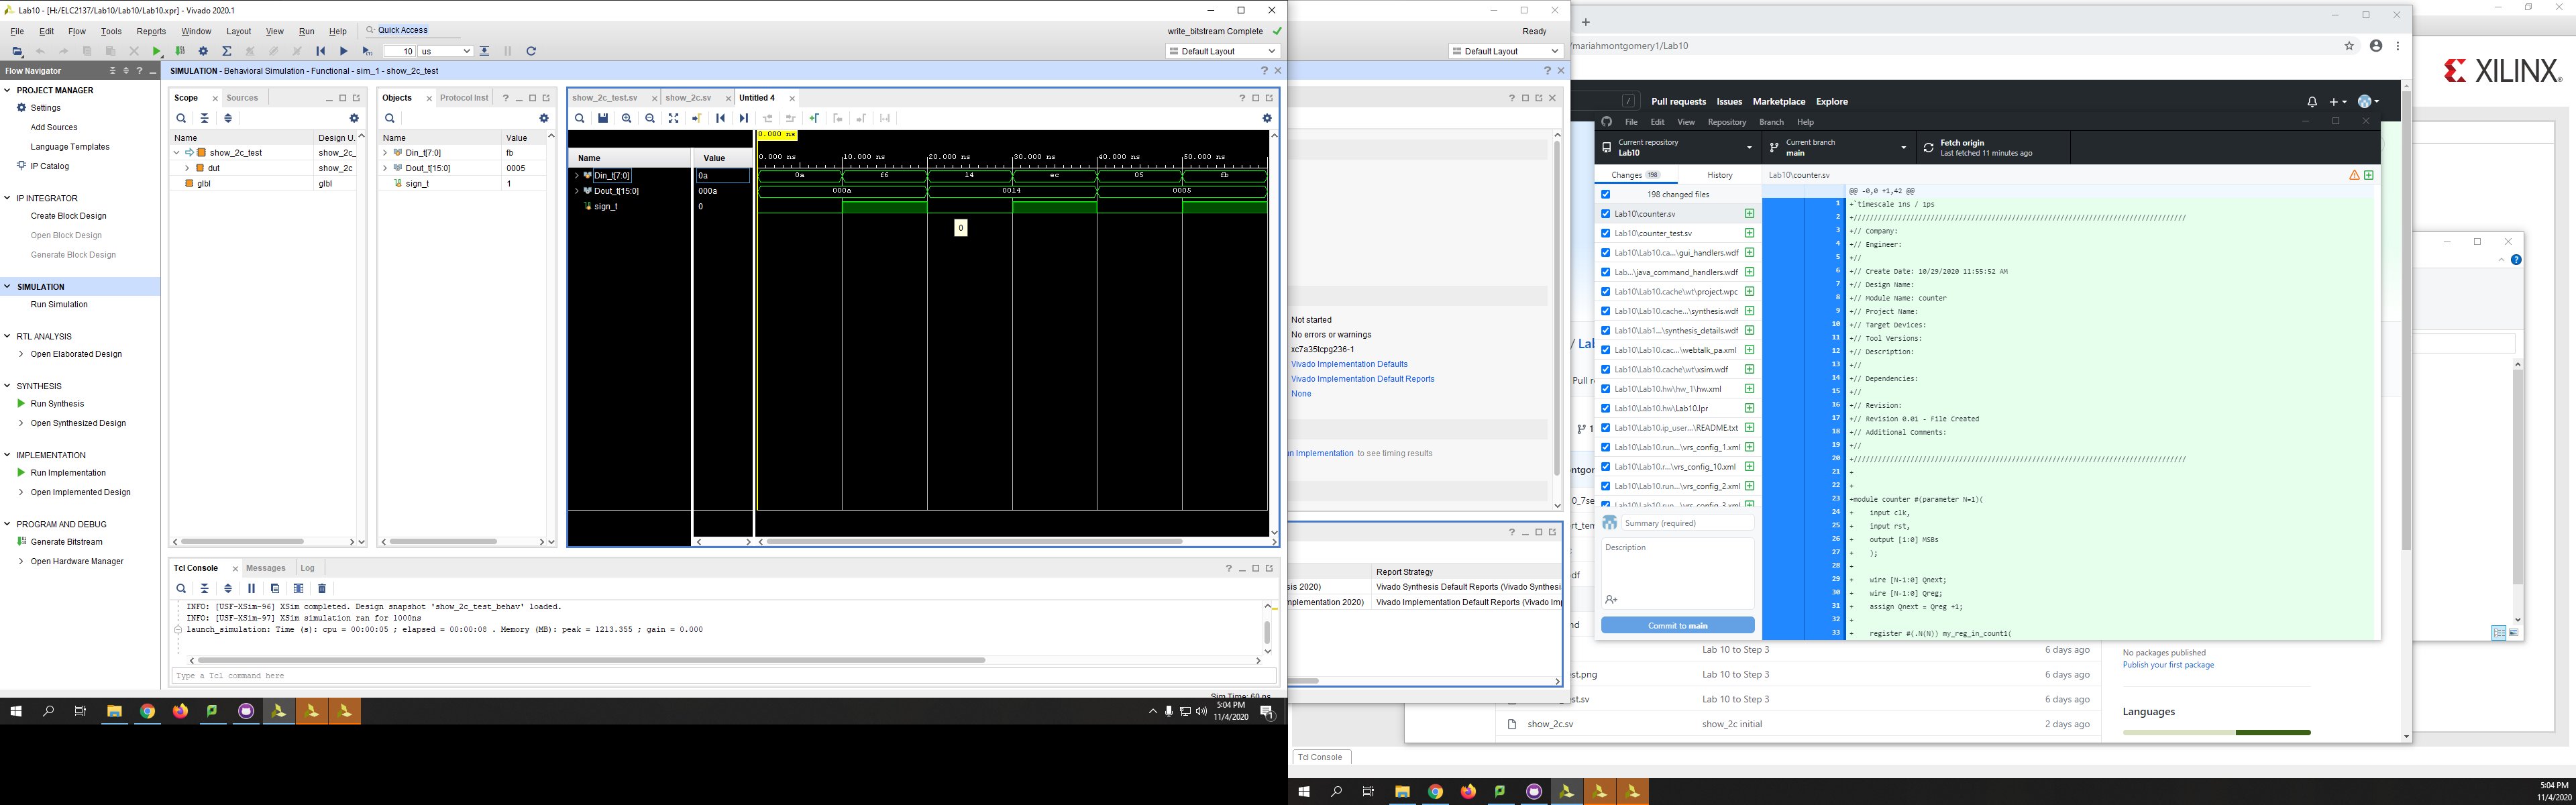
\includegraphics[width=0.8\textwidth, trim= 28.5cm 16cm 68cm 5.5cm, clip]{show_2c_test.PNG}
	\label{fig:Show 2's Complement Test Simulation}
	
	\item Full Strength Four Digits 
	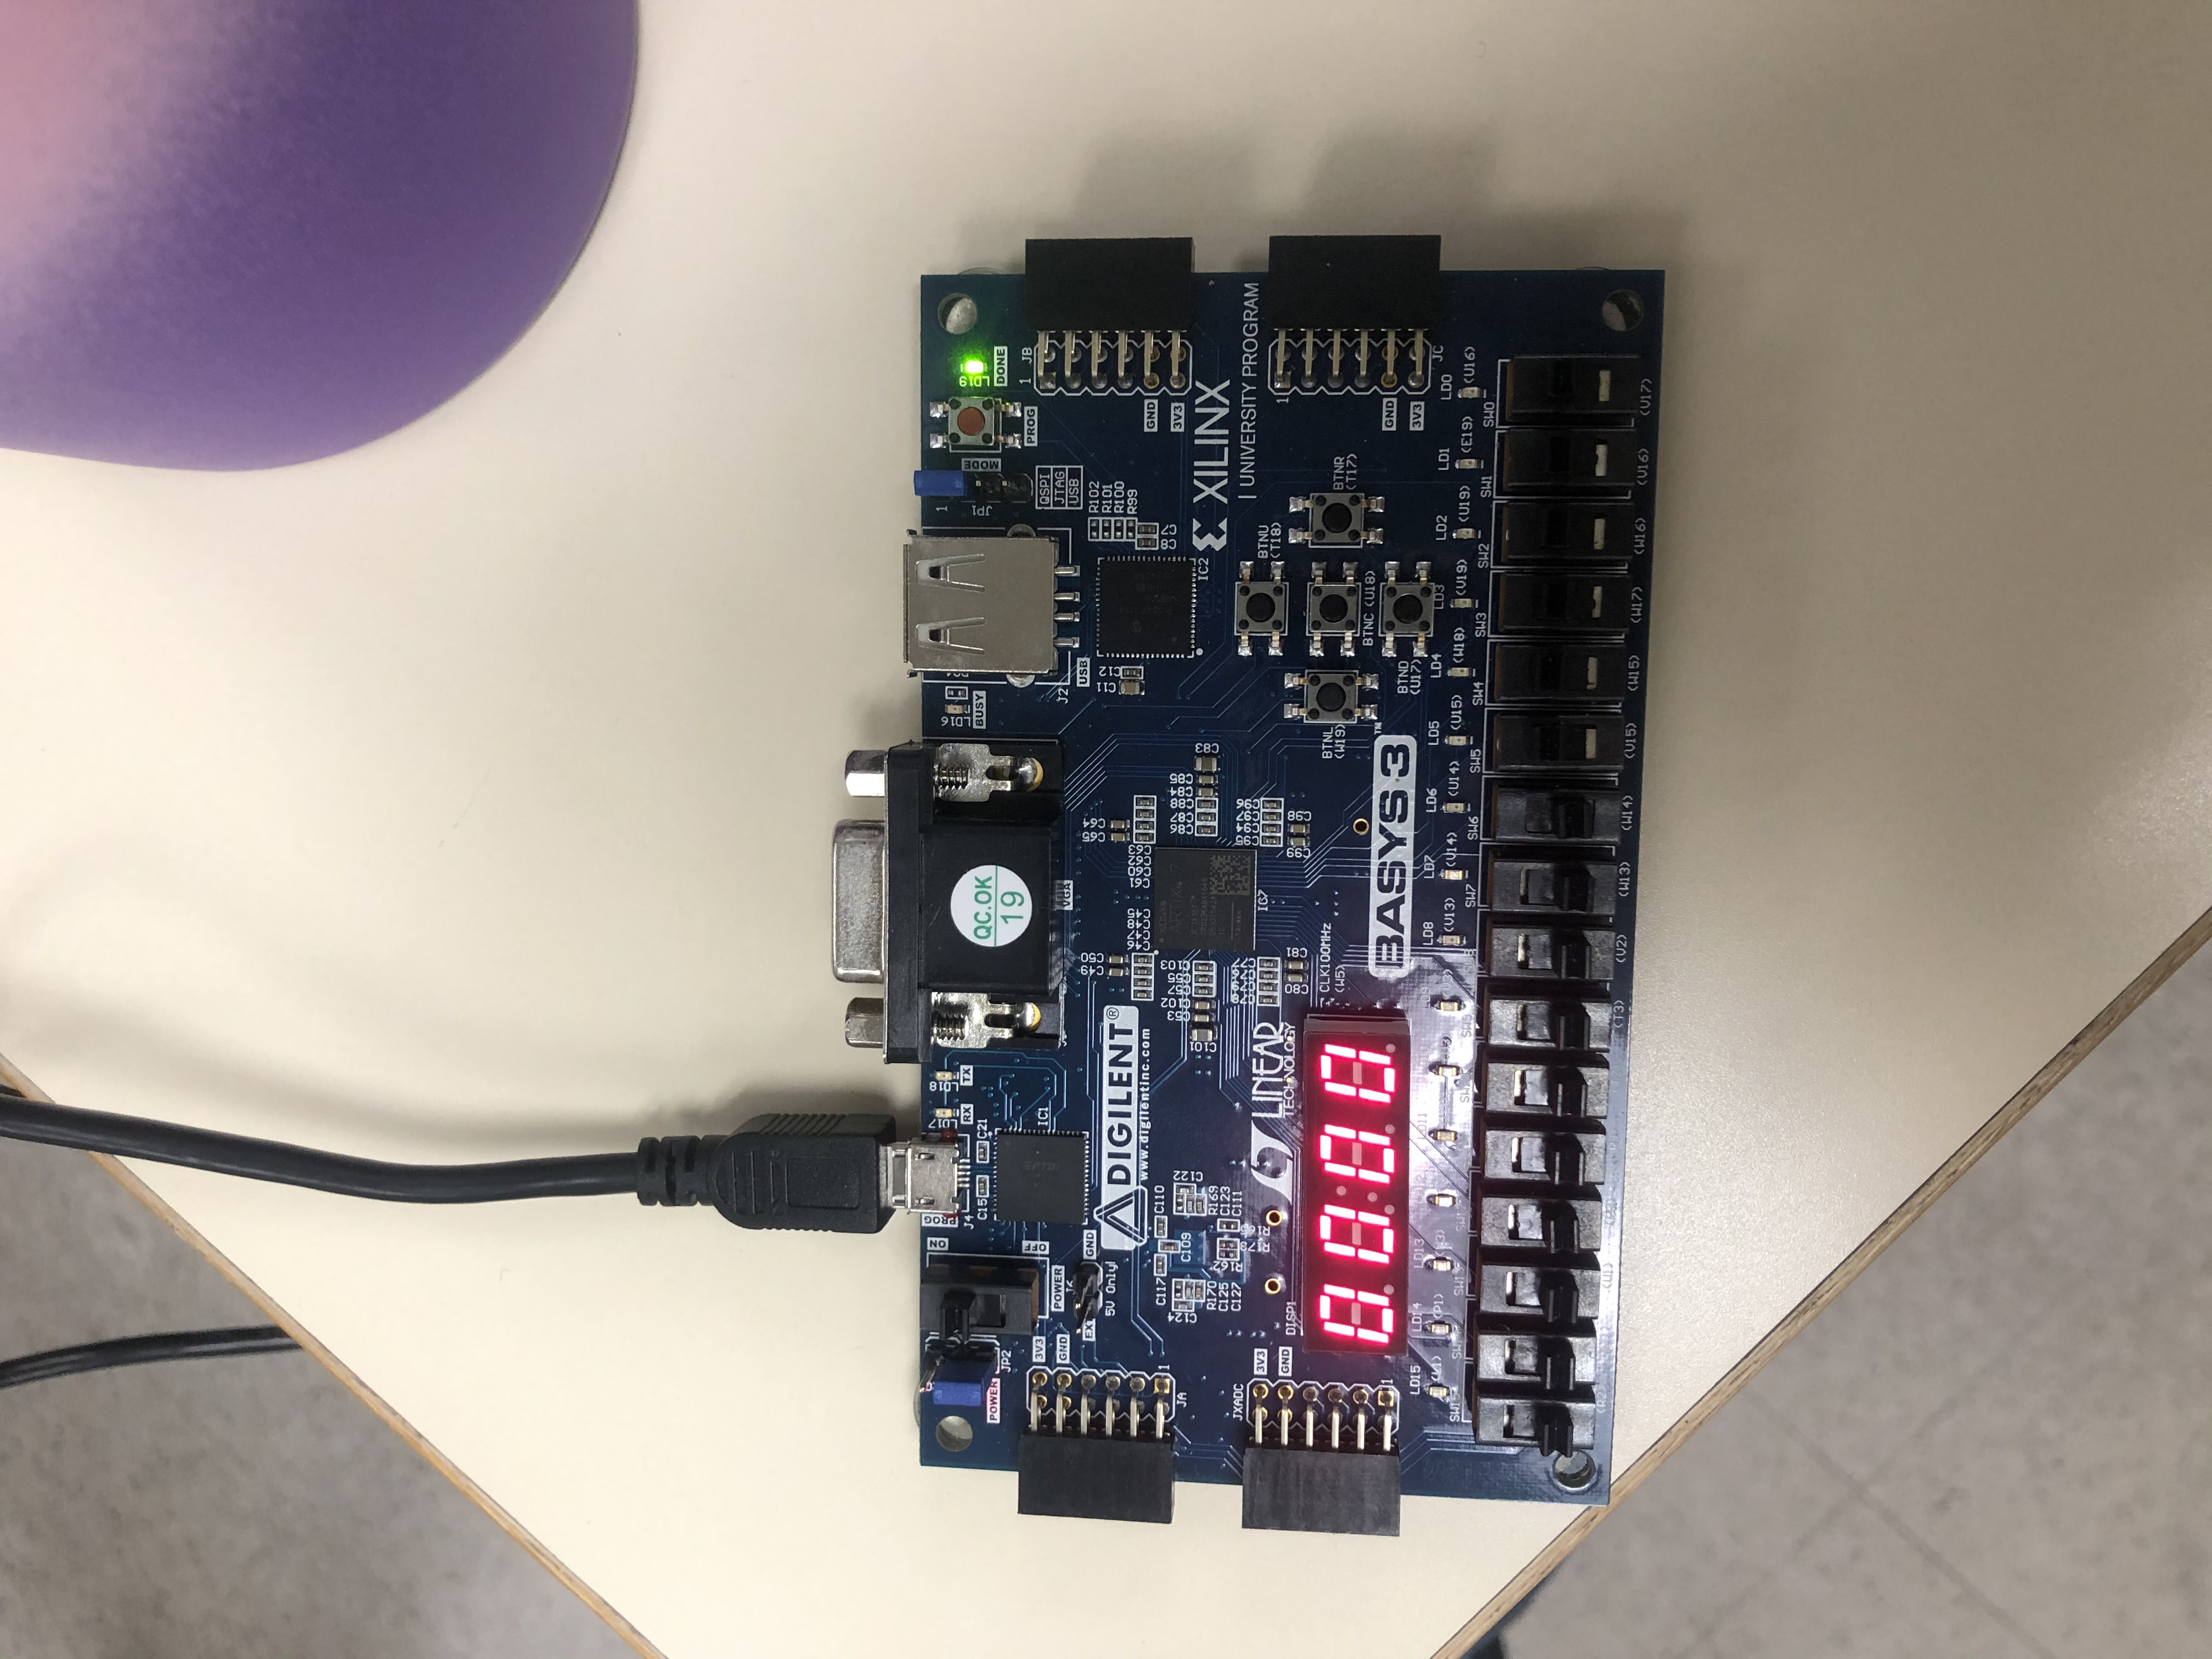
\includegraphics[width=0.8\textwidth, angle = 270]{allZeros.jpg}
	\label{fig:All Zeros}
	
	\item Negative Number Display 
	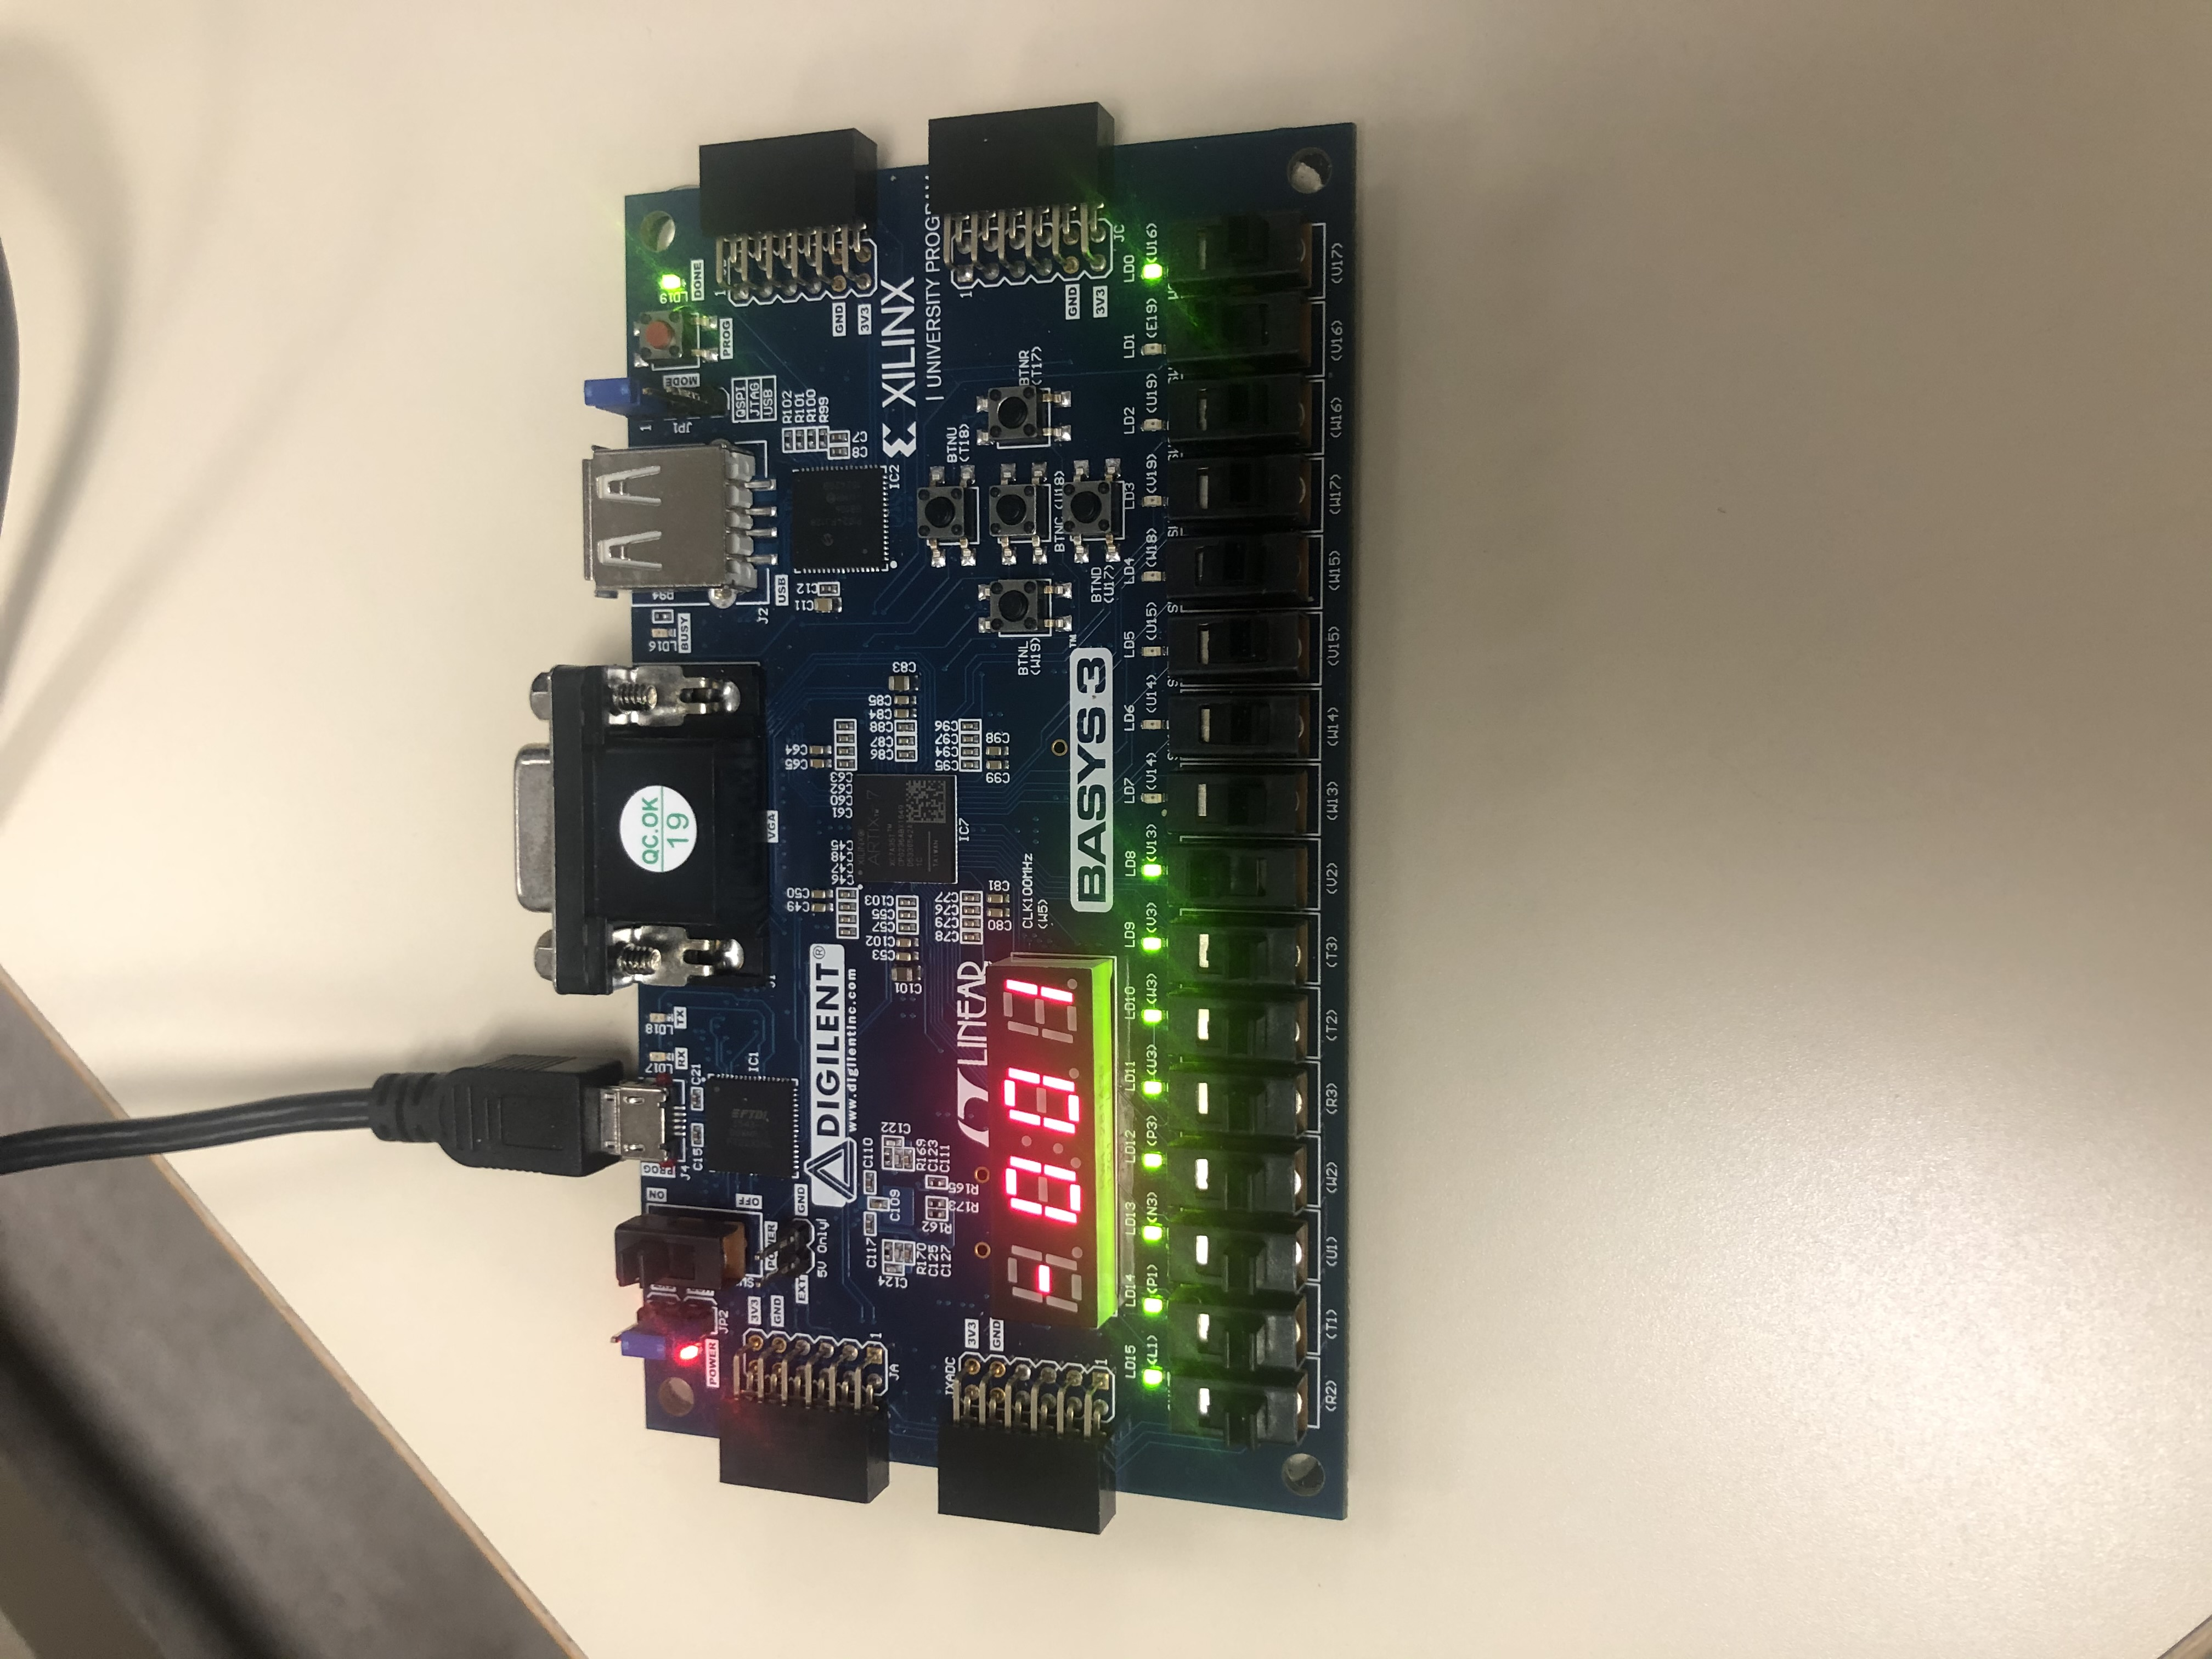
\includegraphics[width=0.8\textwidth, angle = 270]{negativeOne.jpg}
	\label{fig:Negative Number Display}
	
	\item Positive Number Display 
	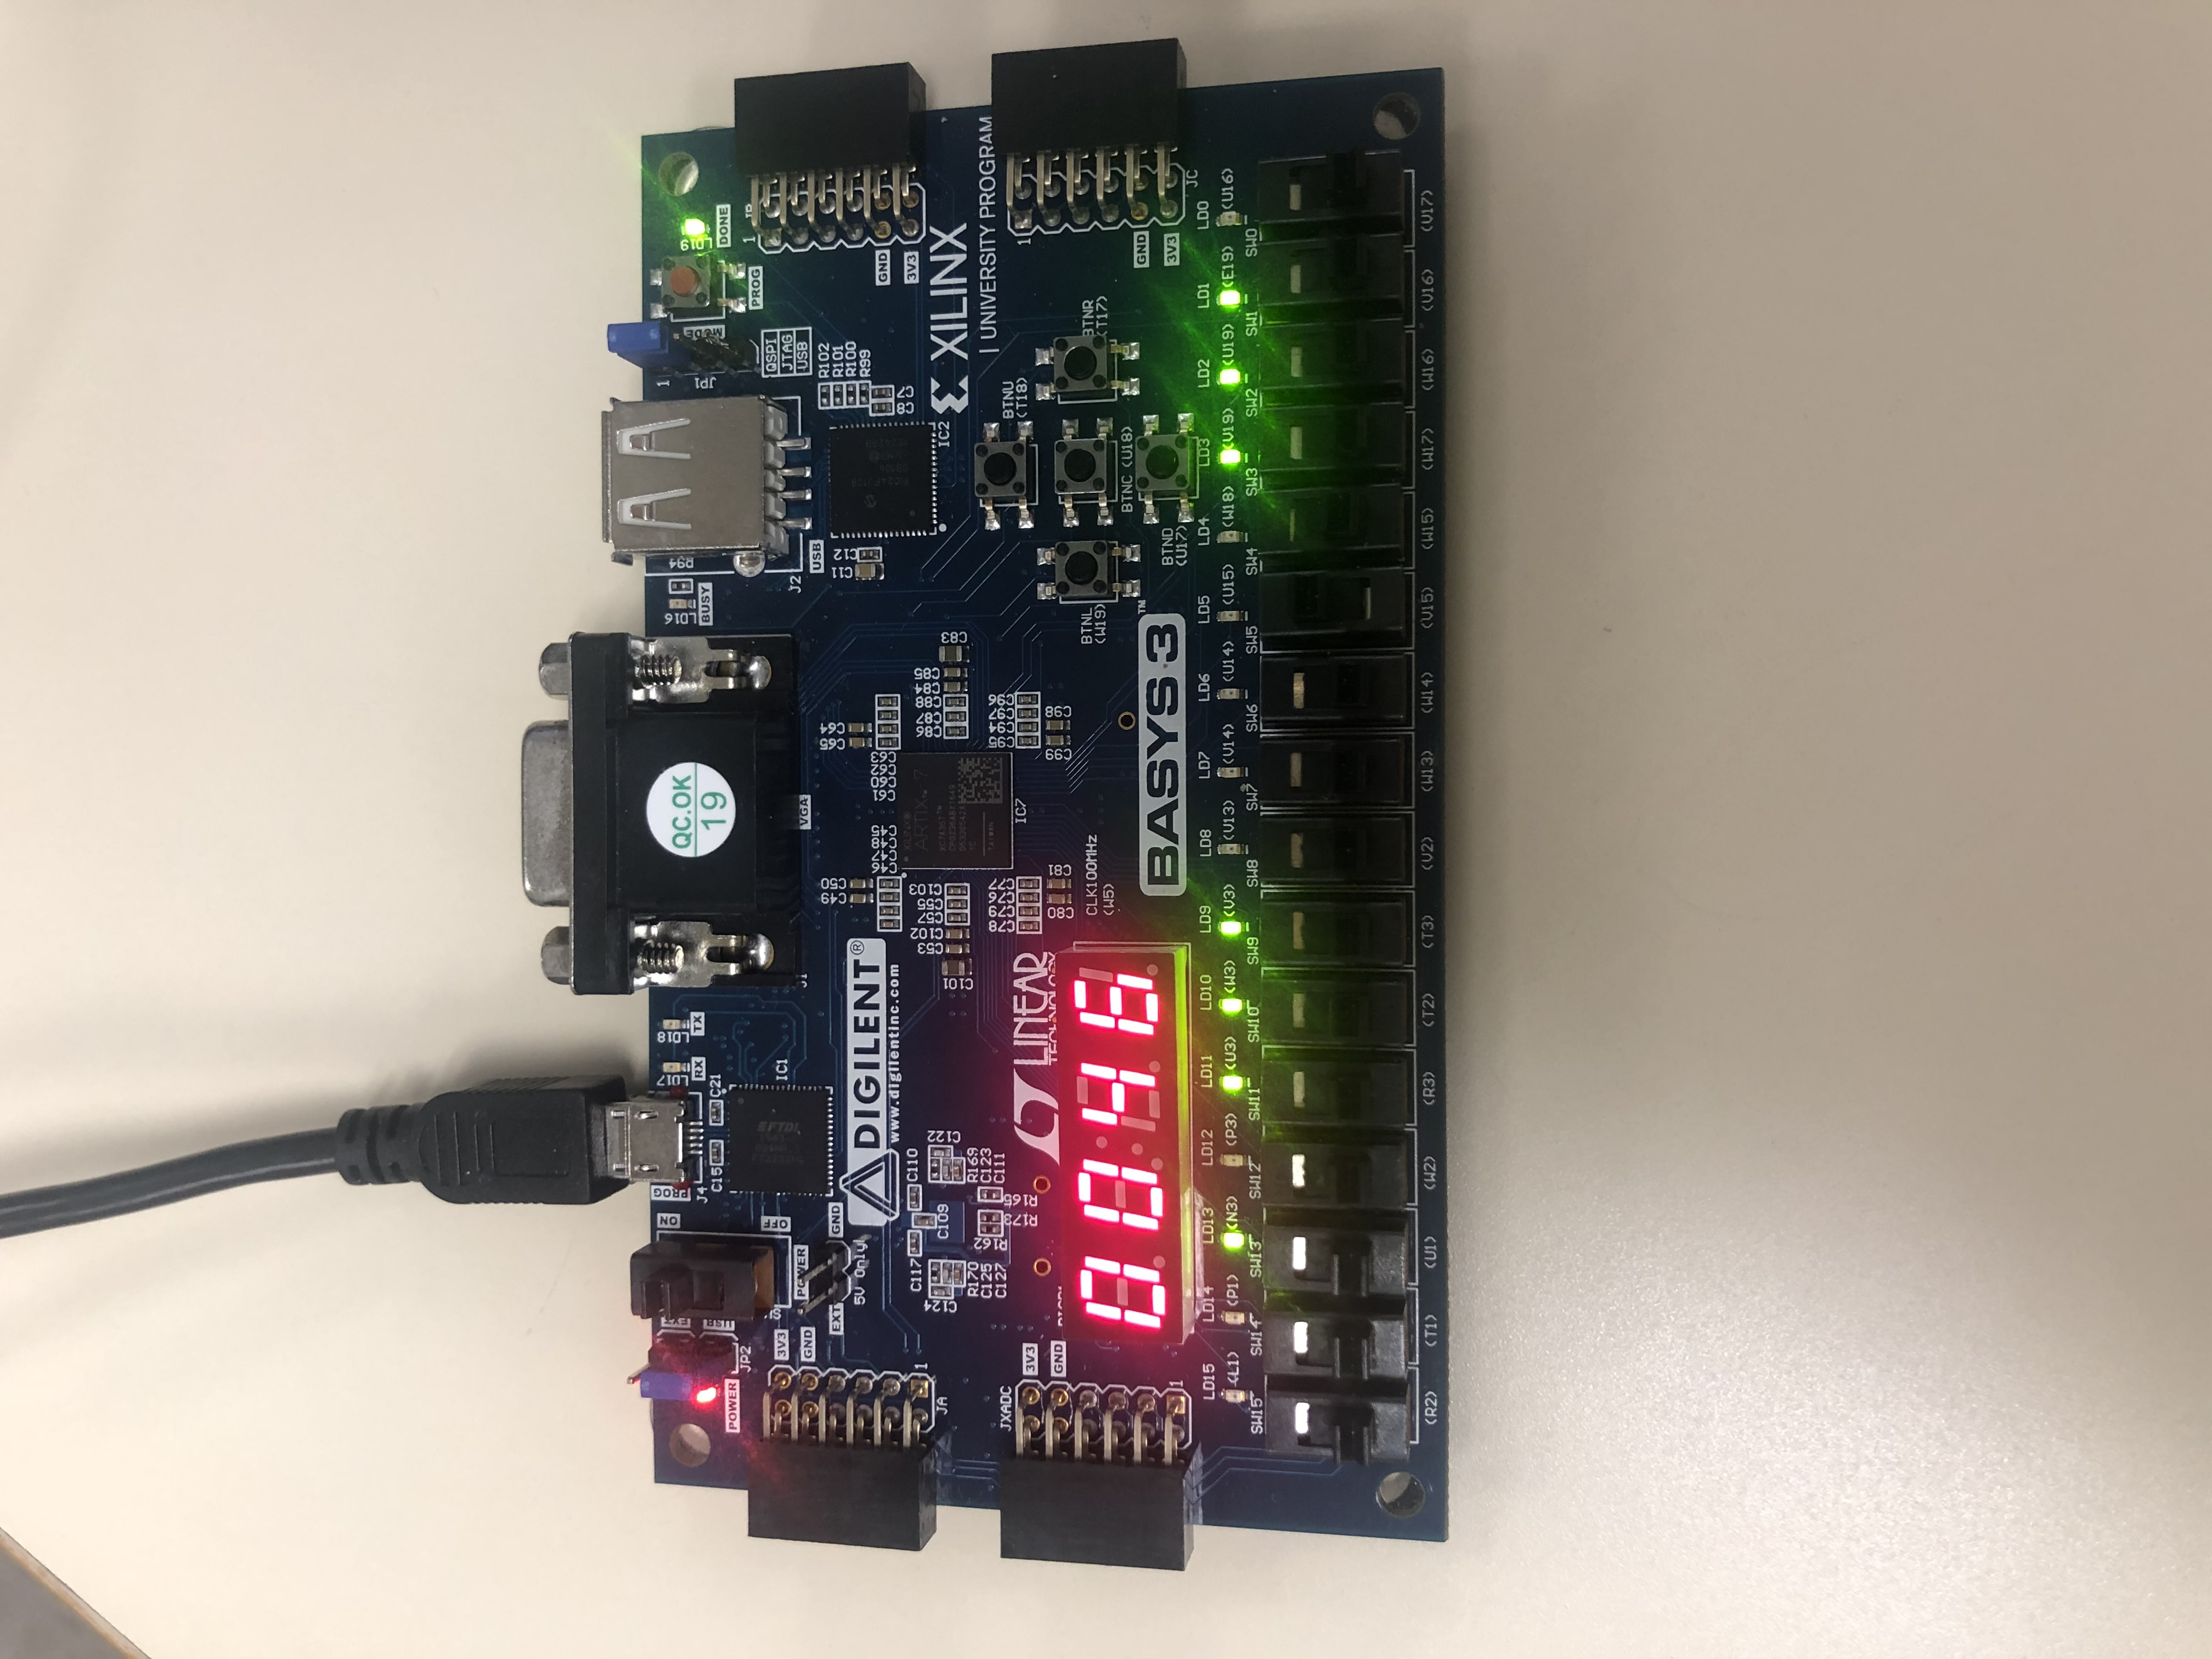
\includegraphics[width=0.8\textwidth, angle = 270]{positveNum.jpg}
	\label{fig:Positive Number Display}
\end{enumerate}


\section*{Code}

\begin{lstlisting}[style=Verilog,caption=Counter, label=counter.sv]
module counter #(parameter N=1)(
	input clk,
	input rst,
	output [1:0] MSBs
	);

	wire [N-1:0] Qnext;
	wire [N-1:0] Qreg;
	assign Qnext = Qreg +1;

	register #(.N(N)) my_reg_in_count1(
		.D(Qnext),
		.clk(clk),
		.en(1),
		.rst(rst),
		.Q(Qreg)
	);

	assign MSBs = Qreg[N-1:N-2];
endmodule
\end{lstlisting}

\begin{lstlisting}[style=Verilog,caption=Counter Test, label=counte_testr.sv]
module counter_test();
	reg clk;
	reg rst_t;
	wire [1:0] MSBs_t;

	counter #(.N(4)) dut(
		.clk(clk),
		.rst(rst_t),
		.MSBs(MSBs_t)
	);

	always begin 
		clk = ~clk; #5;
	end

	initial begin
		clk = 0;
		rst_t = 0; #10;
		rst_t = 1; #3;
		rst_t = 0; #10;
		$finish;
	end 

endmodule

\end{lstlisting}

\begin{lstlisting}[style=Verilog,caption=Wrapper,label=wrapper.sv]
module wrapper(
	input clk,
	input btnC,
	output [6:0] seg,
	output dp,
	output [3:0] an
	);

	wire [1:0] MSBs;

	counter #(.N(20)) my_counter(
		.clk(clk),
		.rst(btnC),
		.MSBs(MSBs)
	);


	sseg4 my_sseg4_lab10(
		.data(16'b0),
		.hex_dec(0),
		.sign(0),
		.digit_sel(MSBs),
		.an(an),
		.dp(dp),
		.seg(seg)
	); 
endmodule
\end{lstlisting}

\begin{lstlisting}[style=Verilog,caption=Show 2's Complement ,label=show_2c.sv]
module show_2c(
	input [7:0] Din,
	output [15:0] Dout,
	output sign
	);
	
	wire [7:0] mux_out;
	wire [7:0] converted_input;
	assign converted_input = ~Din[7:0] + 1;

	mux2 #(.BITS(8)) my_mux2_lab10(
		.in0(Din),
		.in1(converted_input),
		.sel(Din[7]),
		.out(mux_out) 
	);


	assign sign = Din[7];
	assign Dout = {8'b0, mux_out};

endmodule
\end{lstlisting}

\begin{lstlisting}[style=Verilog,caption=Show 2's Complement Test,label=show_2c_test.sv]
module show_2c_test();

	reg [7:0] Din_t;
	wire [15:0] Dout_t;
	reg sign_t;


	show_2c dut(
		.Din(Din_t),
		.Dout(Dout_t),
		.sign(sign_t)
	);

	initial begin
		Din_t = 10; #10;
		Din_t = -10; #10;
		Din_t = 20; #10;
		Din_t = -20; #10;
		Din_t = 5; #10;
		Din_t = -5; #10;
		$finish;
	end 
endmodule
\end{lstlisting}

\begin{lstlisting}[style=Verilog,caption=Top Lab Module,label=top_lab_10.sv]
module top_lab_10(
	input btnU,
	input btnD,
	input [10:0] sw,
	input clk,
	input btnC,
	output [6:0] seg,
	output dp,
	output [3:0] an,
	output [15:0] led
	);

	wire [15:0] lab9Out;
	wire TwocSignOut;
	wire [15:0] TwocMagOut;
	wire [1:0] MSBs;

	top_lab9 my_top_lab9(
		.btnU(btnU),
		.btnD(btnD),
		.btnC(btnC),
		.sw(sw),
		.clk(clk),
		.led(lab9Out)
	);

	show_2c my_show_2c(
		.Din(lab9Out[15:8]),
		.Dout(TwocMagOut),
		.sign(TwocSignOut)
	);

	counter #(.N(20)) my_counter(
		.clk(clk),
		.rst(btnC),
		.MSBs(MSBs)
	);


	sseg4 my_sseg4_lab10(
		.data(TwocMagOut),
		.hex_dec(sw[15]),
		.sign(TwocSignOut),
		.digit_sel(MSBs),
		.an(an),
		.dp(dp),
		.seg(seg)
	); 

	assign led = lab9Out;

endmodule
\end{lstlisting}

\end{document}
